\section{Hardware Architecture}
\label{sec:arch}
\subsection{Overview}
An overview of \spatten is shown in Figure~\ref{fig:arch_overview}. 
To support token/head pruning, a novel \topk engine (Figure~\ref{fig:topk}) is designed to rank the token/head importance. Pruning reduces computation and memory traffic but incurs random access. Thus, a crossbar is applied to process the addresses, keep each memory channel busy, and increase the bandwidth utilization rate. To support progressive \lowprec, we implement an on-chip \bitwidth converter to handle the splits of fetched bits and concatenations of MSBs and LSBs.


\spatten processes attention head by head and query by query, thus well balancing the pruning granularity and parallelism. One query of a head is fed to the pipeline at a time, enabling token pruning in both head-wise and layer-wise granularity. Inner-head parallelism can keep all on-chip computation resources busy, so no need for inter-head parallelism. In the summarization stage, K and V that survive cascade token pruning are fetched to the on-chip SRAM and will be \emph{reused} across multiple queries. In the generation stage, the Q is a single vector, so there is no reuse of K and V, and no need to store them in the on-chip SRAM.


For each fetched Q, the \topk engine (Figure~\ref{fig:topk}) first ranks the token importance scores and get $k$ most important Ks. A data fetcher then computes the Ks' addresses and feeds them to a 32$\times$16 crossbar for 16 HBM channels. It then gets data back through a reverse 16$\times$32 crossbar to preserve the correct order. 
Q and K are processed by a matrix-vector multiplication module (Figure~\ref{fig:qxk}) to get the attention scores. 
A Softmax module (Figure~\ref{fig:softmax} left) then processes the attention scores to get attention probabilities, and sends them to the progressive quantization module (Figure~\ref{fig:softmax} right) to decide whether LSBs are required. The probabilities are also sent to the token importance score accumulator to perform accumulations.
After that, the local Value pruning \topk engine gets the probabilities, computes $k$ most locally important Vs, and sends their indices to the data fetcher. Finally, the remaining probabilities are multiplied with fetched V, getting attention outputs. After computing one head, the head importance score will be accumulated. After finishing all heads in a layer, a top-k module prunes unimportant heads, which will not be computed in any following layers. 

Our dataflow guarantees to avoid fetching pruned tokens and value vectors, thus bringing DRAM access reductions. The critical path (module 6,7,8,10,11) is fully pipelined. The accumulation of token/head importance scores and token/head top-k are performed \emph{in parallel} with the critical path. For module 3 branches, when multiple sources of Q/K/V requests come simultaneously, the fetcher processes requests one by one and sends addresses to FIFOs. The branches after module 8/11 send $attention\_prob/attention\_out$ to accumulators and the next corresponding computation module simultaneously. For the module 9 branch, if LSB is required, it discards $attention\_prob$ and initiates recomputation; then modules 10 and 11 will be idle, waiting for recomputed attention probabilities. For module 10 branch, fetching un-pruned V from DRAM is part of the coarse-grained pipeline.

\begin{figure}[t]
    \centering
    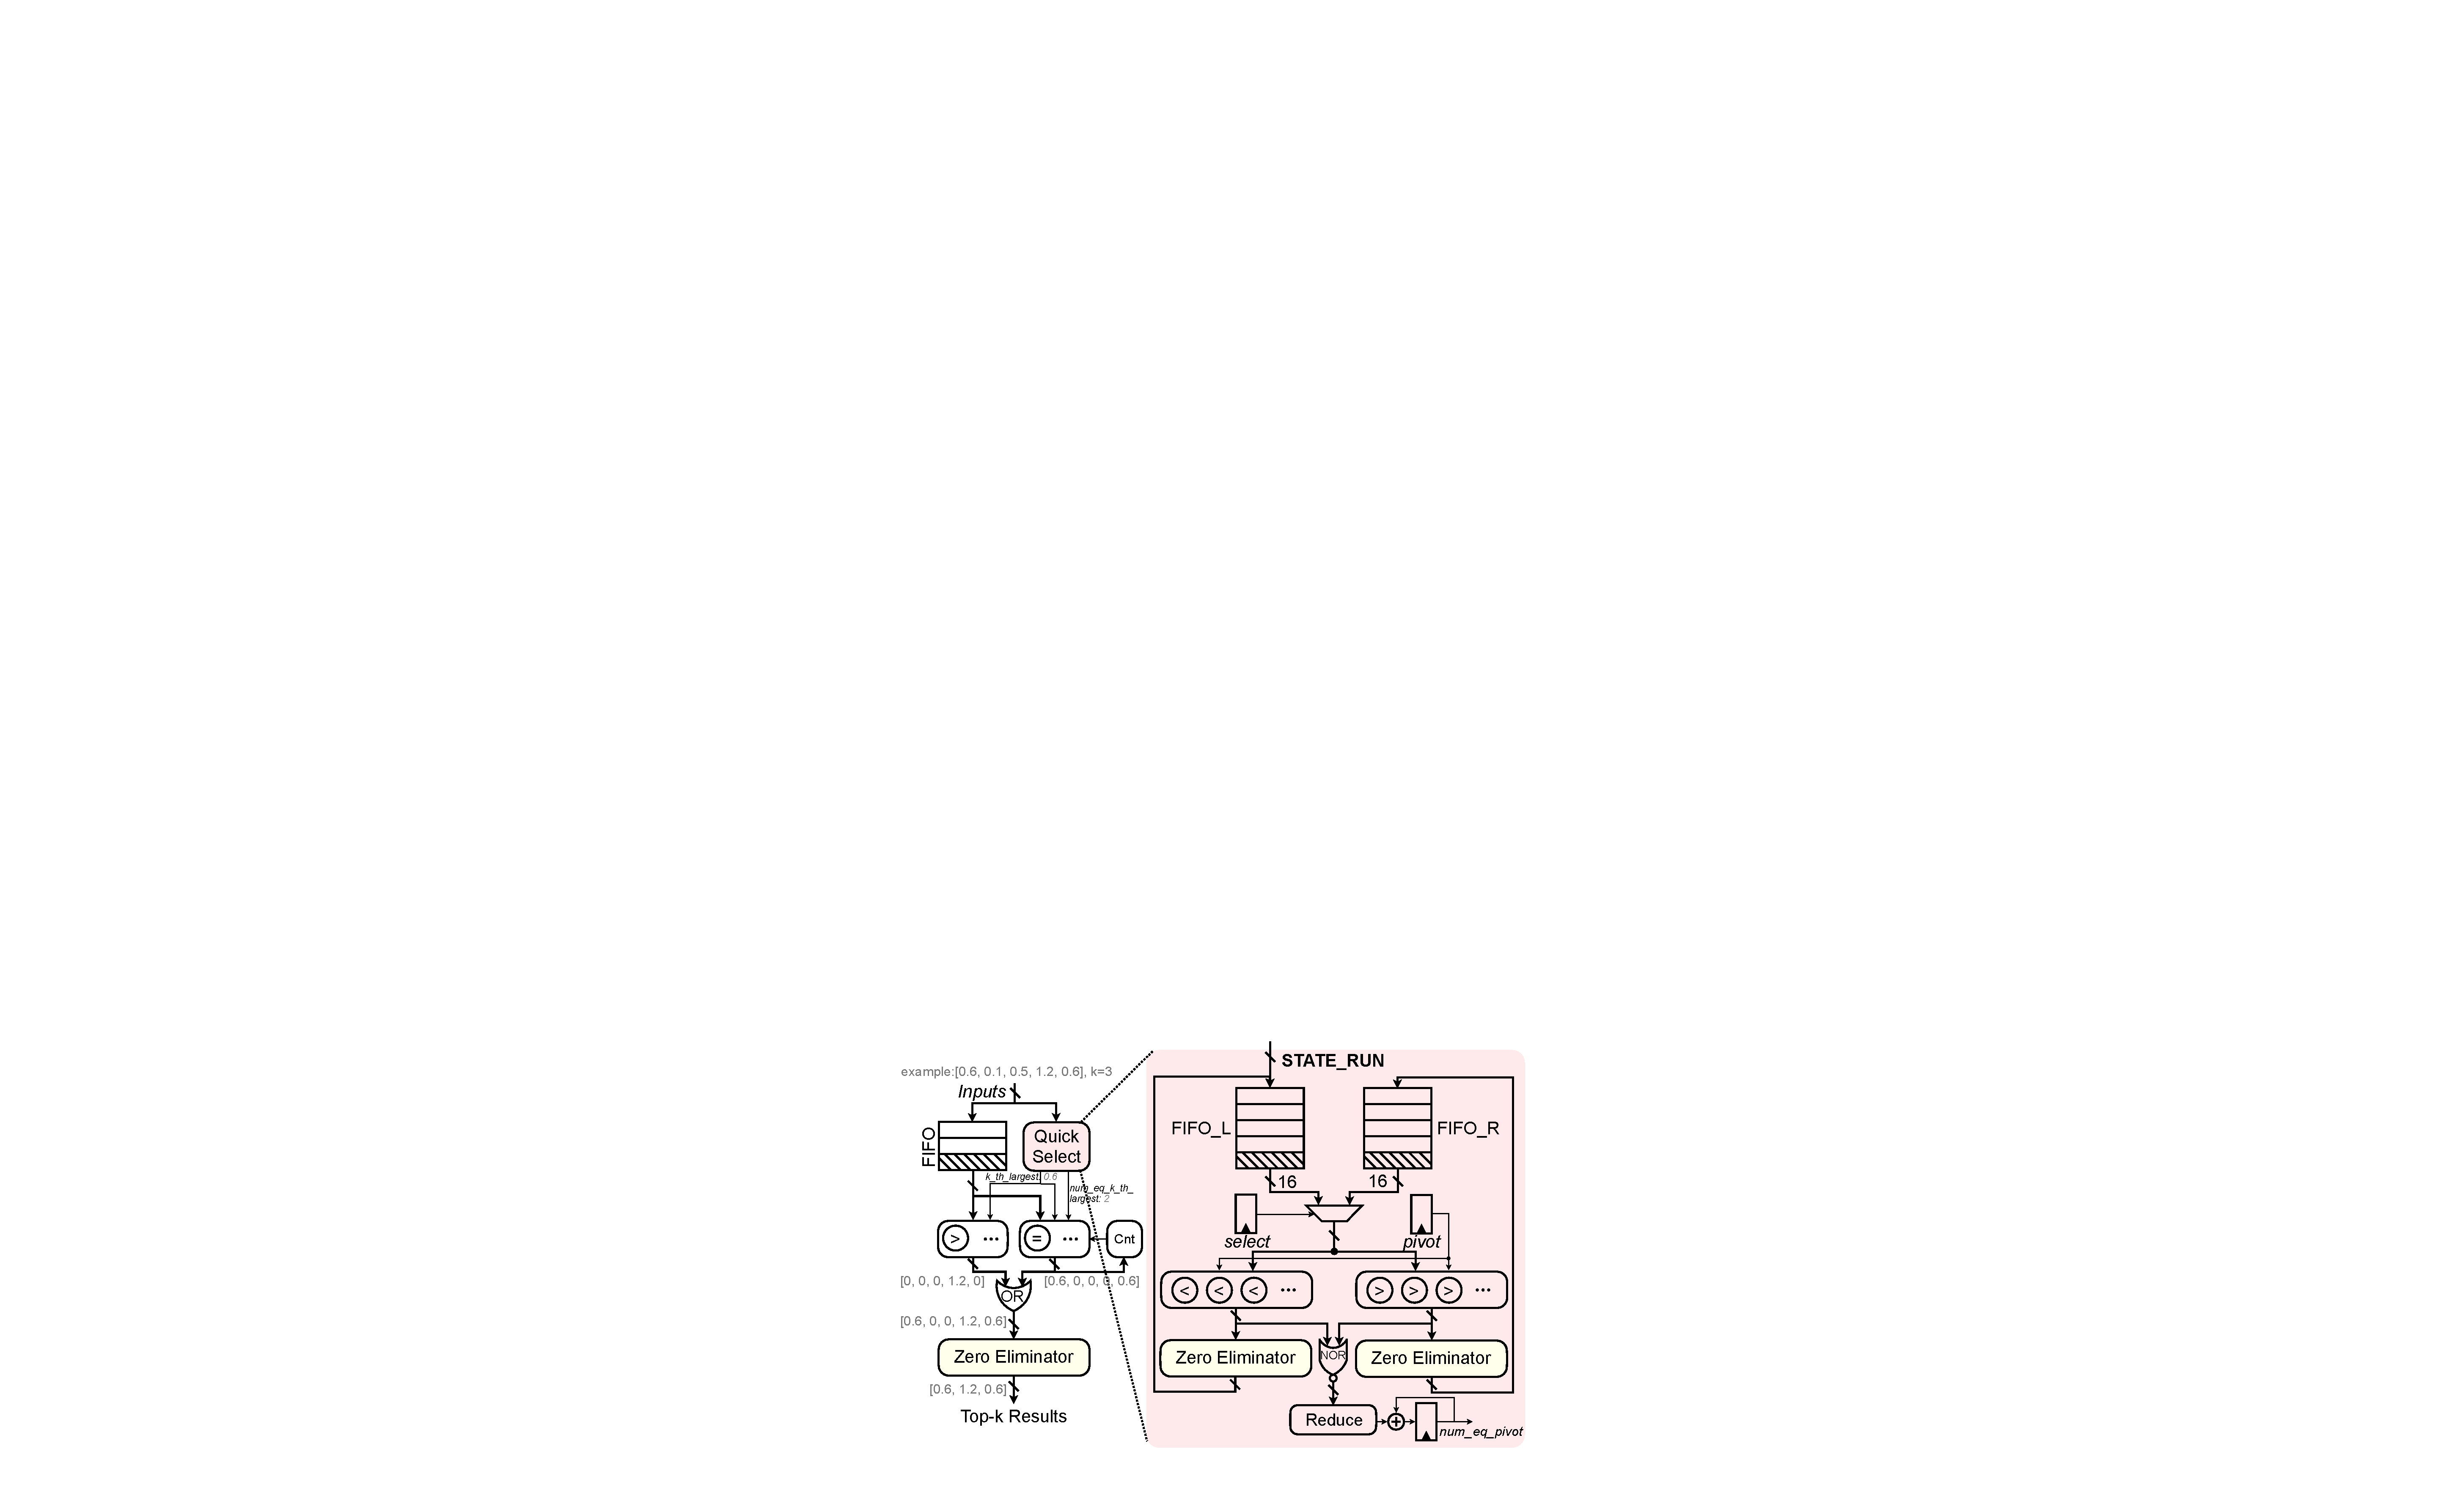
\includegraphics[width=\columnwidth]{figures/topk.pdf}
     \vspace{-10pt}
    \caption{High Parallelism \topk Engine.
    }
     \vspace{-10pt}
    \label{fig:topk}
\end{figure}

The on-chip memory system has two main SRAMs for Key and Value, 196KB each in module 7 and module 11. They store K and V from QKV Fetcher. Since we process queries one by one, the Q vector is stored in registers. We also have 32 64-depth$\times$8B address FIFOs after QKV fetcher and 32 64-depth$\times$16B data FIFOs before bitwidth converter.

\begin{figure}[t]
    \centering
    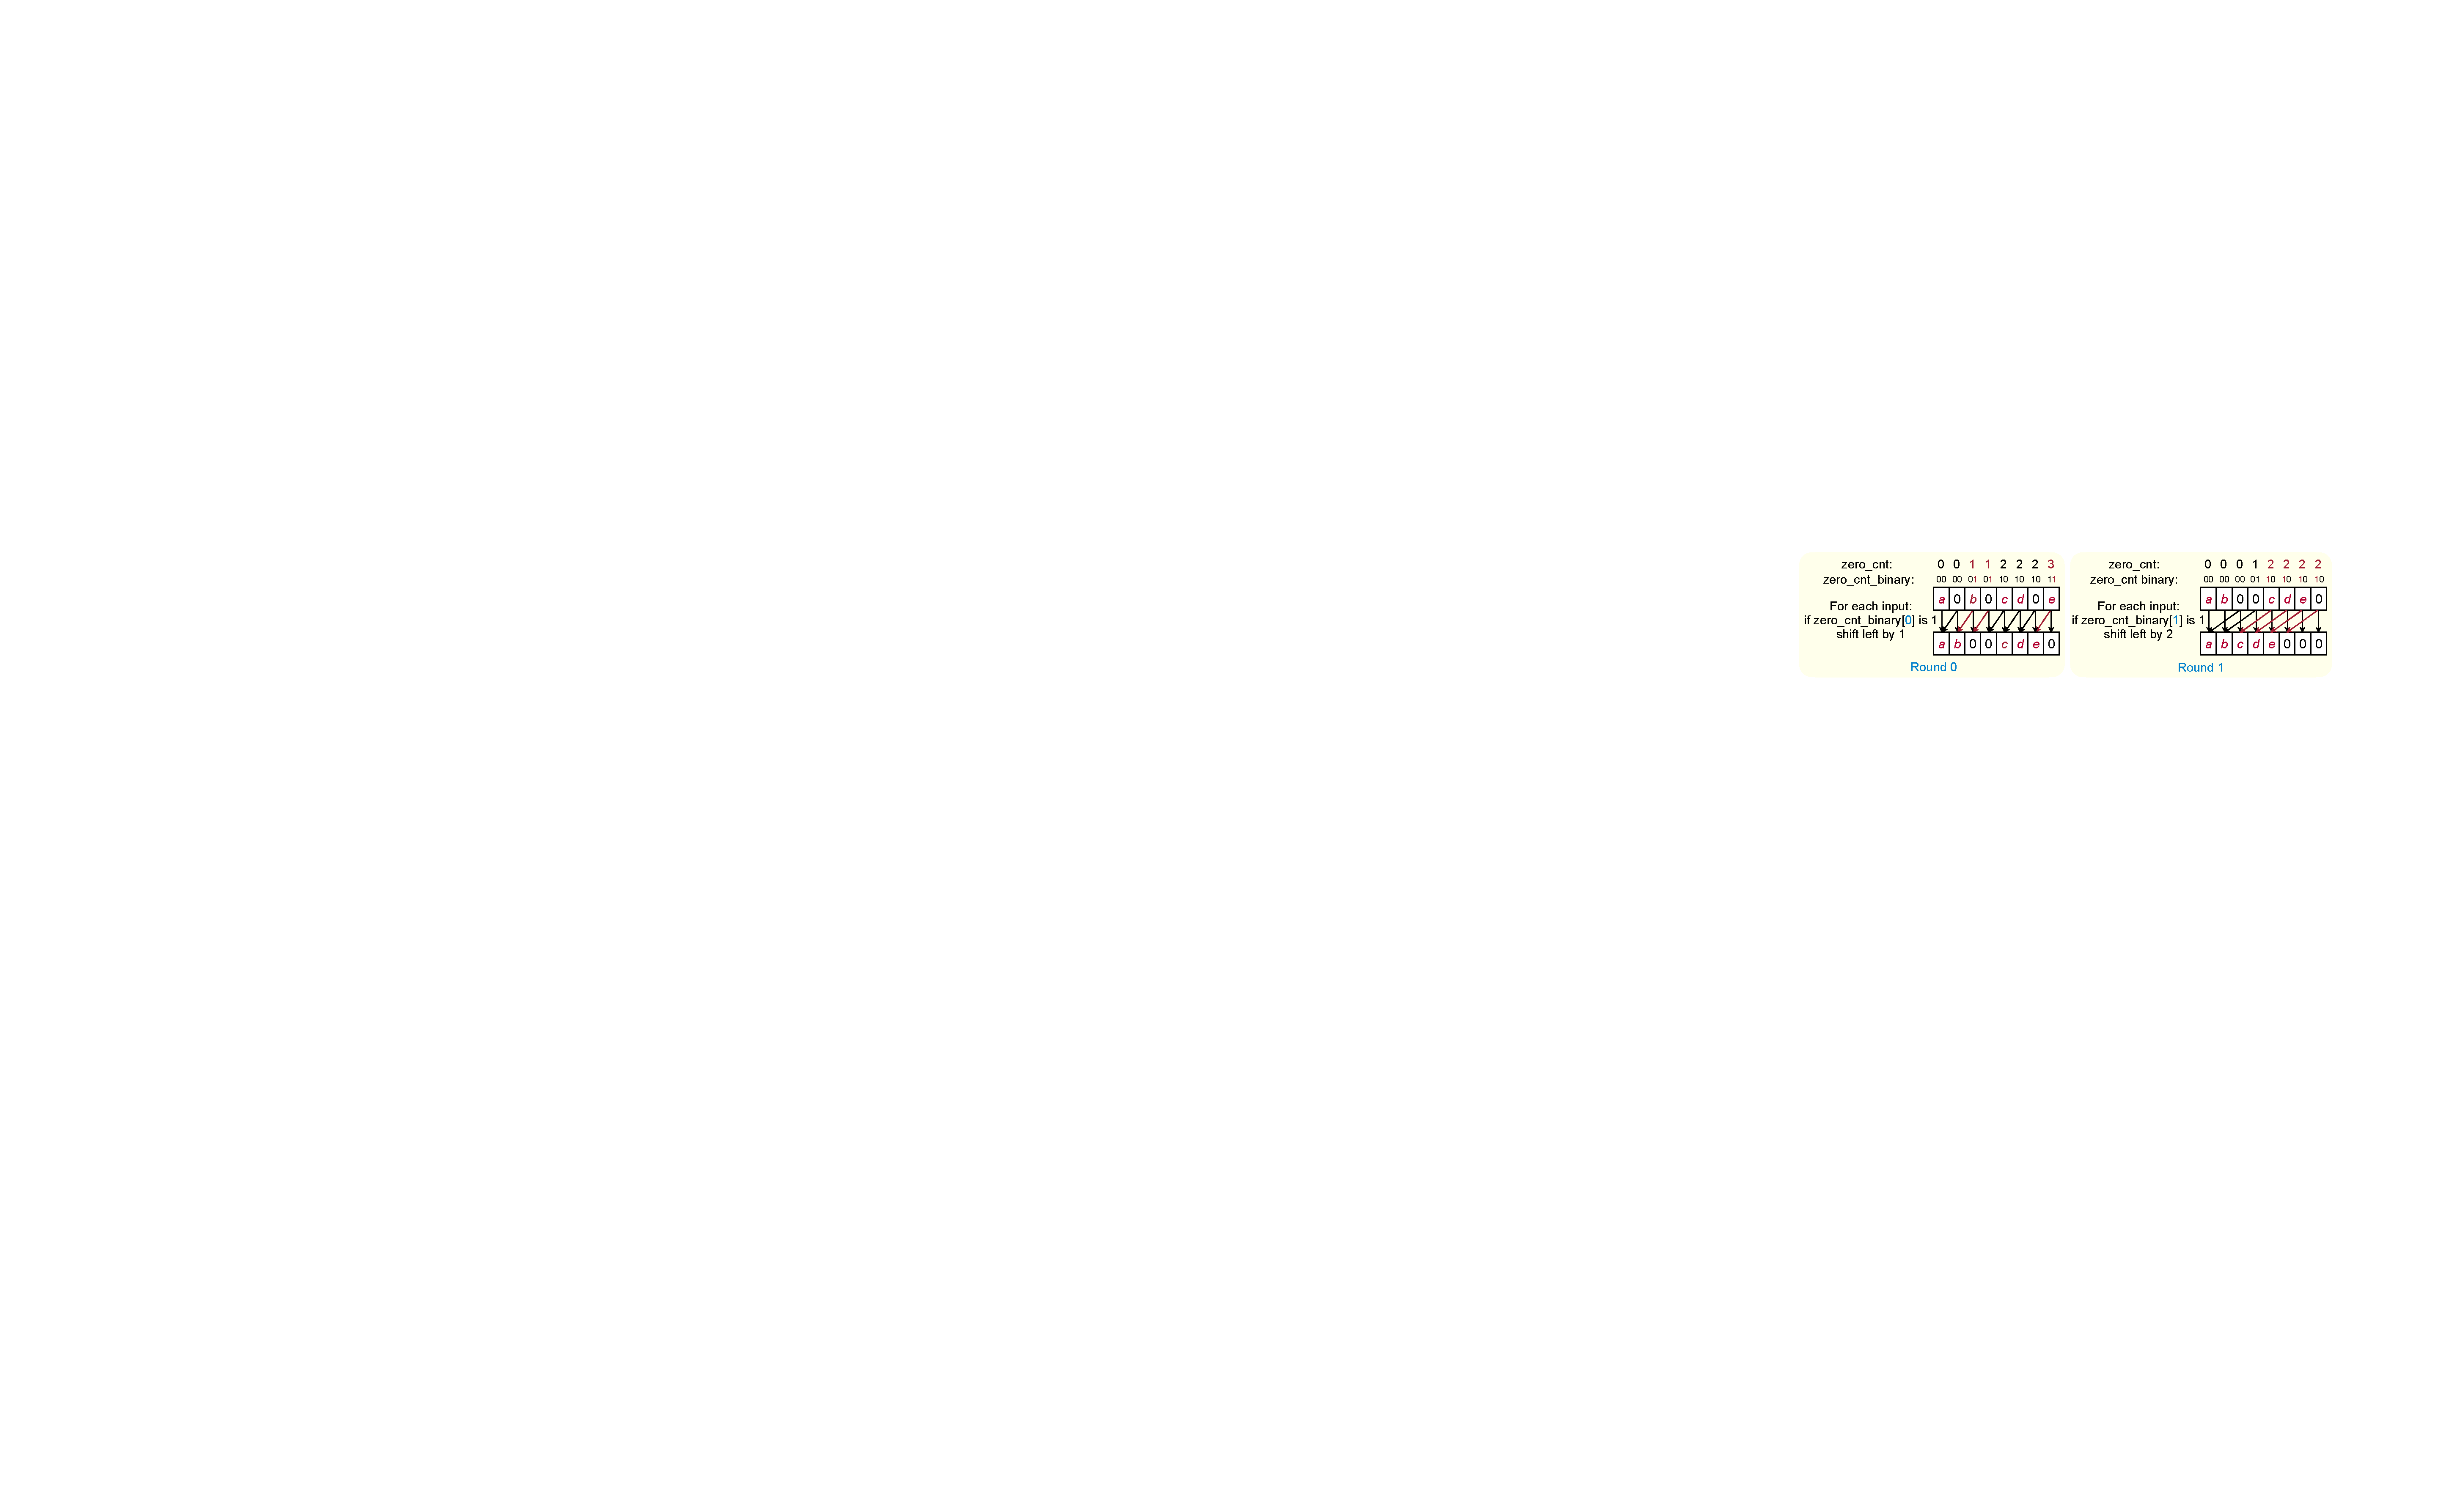
\includegraphics[width=\columnwidth]{figures/ze.pdf}
     \vspace{-20pt}
    \caption{Zero Eliminator. A zero eliminator of $n$ elements has $\log n$ stages.}
     \vspace{-20pt}
    \label{fig:ze}
\end{figure}

\begin{algorithm}[!t]
\footnotesize{
\SetKwInOut{Input}{Input}
    \textbf{Input:} Top-k $k$, Data vector $inputs$; \\
    FIFO\_L, FIFO\_R depth: 64; FIFO $=$ [FIFO\_L, FIFO\_R]; \\
    Initialize FIFO\_L with $inputs$, FIFO\_R $= \phi$; \\
    $target = k$, $num\_eq\_pivot = 0$;\\
    \SetAlgoLined
    \textbf{START:} \\
    \uIf{ $\mathrm{size(FIFO\_R)} + num\_eq\_pivot \le target$ }{
    \tcc{ the selected pivot is too large}
    $target = target - \mathrm{size(FIFO\_R)}-num\_eq\_pivot$; \\
    FIFO\_R $ =\phi$; $select = 0$; $pivot = $ FIFO\_L[rand]; \\
    Goto \textbf{STATE\_RUN};\\
    
    }
    
    \uElseIf{$\mathrm{size(FIFO\_R)} > target$}{
    \tcc{ the selected pivot is too small}
    FIFO\_L $=\phi$; $select = 1$; $pivot = $ FIFO\_R[rand]; \\
    Goto \textbf{STATE\_RUN}; \\
    }
    
    \Else{ \tcc{
    $\mathrm{size(FIFO\_R)} \le target$
    $\mathrm{size(FIFO\_R)} + num\_eq\_pivot > target $
    }
    $k\_th\_largest = pivot$; \\ $num\_eq\_k\_th\_largest = target$-size(FIFO\_R); \\
    \textbf{Output:} [$k\_th\_largest, num\_eq\_k\_th\_largest$]; \\
    }
    
    \colorbox{topkcolor}{\vbox{
    \textbf{STATE\_RUN:} (Figure \ref{fig:topk} Right) \\
    \tcc{items smaller than pivot $\rightarrow$ FIFO\_L \\
    items larger than pivot $\rightarrow$ FIFO\_R}
     $num\_eq\_pivot = 0$; \\
    \For{$i = 0 \mathbf{ \ to \ } \mathrm{size(FIFO} [select])-1$}{
    Pop FIFO[$select$] as $item$;\\
    \uIf{$item < pivot$}{
    Push $item$ to FIFO\_L;\\
    }
    
    \uElseIf{$item > pivot$}{Push $item$ to FIFO\_R;\\}
    \Else{ \tcc{$item == pivot$}
    $num\_eq\_pivot = num\_eq\_pivot + 1$;\\}
    }
    Goto \textbf{START};
    }}
    
    
    
    
    \caption{\topk Engine}
    }
    \label{algorithm:topk}

\afterpage{\global\setlength{\textfloatsep}{\oldtextfloatsep}}

\end{algorithm}




\subsection{Top-k Engine}
To support cascade token/head pruning and local value pruning, we need to find the top $k$ elements of an array. A na\"ive solution is to use a sorter to sort the original array and directly output the first $k$ elements. However, it needs $O(n\cdot \log n)$ time complexity and $O(n\cdot \log^2n)$ space sorting network, and also completely randomizes data fetching.
Instead, we design a novel \topk engine (Figure~\ref{fig:topk}) with a quick-select module to find the $k^{\mathrm{th}}$ largest element as a threshold to filter the input array. It has much lower time complexity ($O(n)$ on average) and keeps the original order of inputs.
The engine leverages a randomly chosen pivot to partition the input array into two parts: elements smaller or larger than the pivot. It has two FIFOs, FIFO\_L and FIFO\_R, to store the partitioned arrays. An array to be partitioned will be fed into two comparator arrays and compared with the pivot. The left/right comparator array only preserves elements smaller/larger than the pivot. Others will be set to zeros and eliminated by a zero eliminator. Quick-select runs iteratively until the $k^{\mathrm{th}}$ largest element is found. The control logic is in Algorithm~\ref{algorithm:topk}.
Afterwards, the $k^{\mathrm{th}}$ largest element is used to filter the input array, which is buffered in another FIFO (Figure~\ref{fig:topk} left) before the quick-select process. The filtered outputs will be processed by another zero eliminator to finally get the top-k elements.
It can be easily scaled up with more comparators. In \spatten, we apply 16 comparators in each array to make it not the whole pipeline's bottleneck. Since the frequency of head pruning is much lower than token pruning and local Value pruning, we reuse the token pruning \topk engine for head pruning. Therefore, we have two \topk engines in \name architecture.


\subsection{Zero Eliminator}
We design an innovative logic for the zero eliminator, which first uses a prefix sum module to calculate the number of zeros before each element $zero\_cnt$. These $zero\_cnt$ will guide a logN layer shifter to shift the input array by 1, 2, 4, ... positions. In the $n^{\mathrm{th}}$ layer, whether to shift an element is determined by the $n^{\mathrm{th}}$ bit of its corresponding $zero\_cnt$. An example is illustrated in Figure~\ref{fig:ze}.


The top-k engine equipped with zero-eliminators has much higher parallelism than a direct implementation of quick select. Without high parallelism, the performance will be bottlenecked by finding top-k. In Figure~\ref{fig:perfbreak}, we show that SpAtten with a parallelized top-k engine can achieve 3$\times$ speedup over a baseline top-k engine with parallelism=1. We also compare a regular full sorting unit (a Batcher's Odd-Even Sorter~\cite{10.5555/280635} to perform merge-sort) to the worst case of the top-k engine (selecting the median) with an input length of 1024. Experimental results show that we can achieve 1.4\x higher throughput with 3.5\x smaller power consumption over the full sorting unit.


\begin{figure}[t]
    \centering
    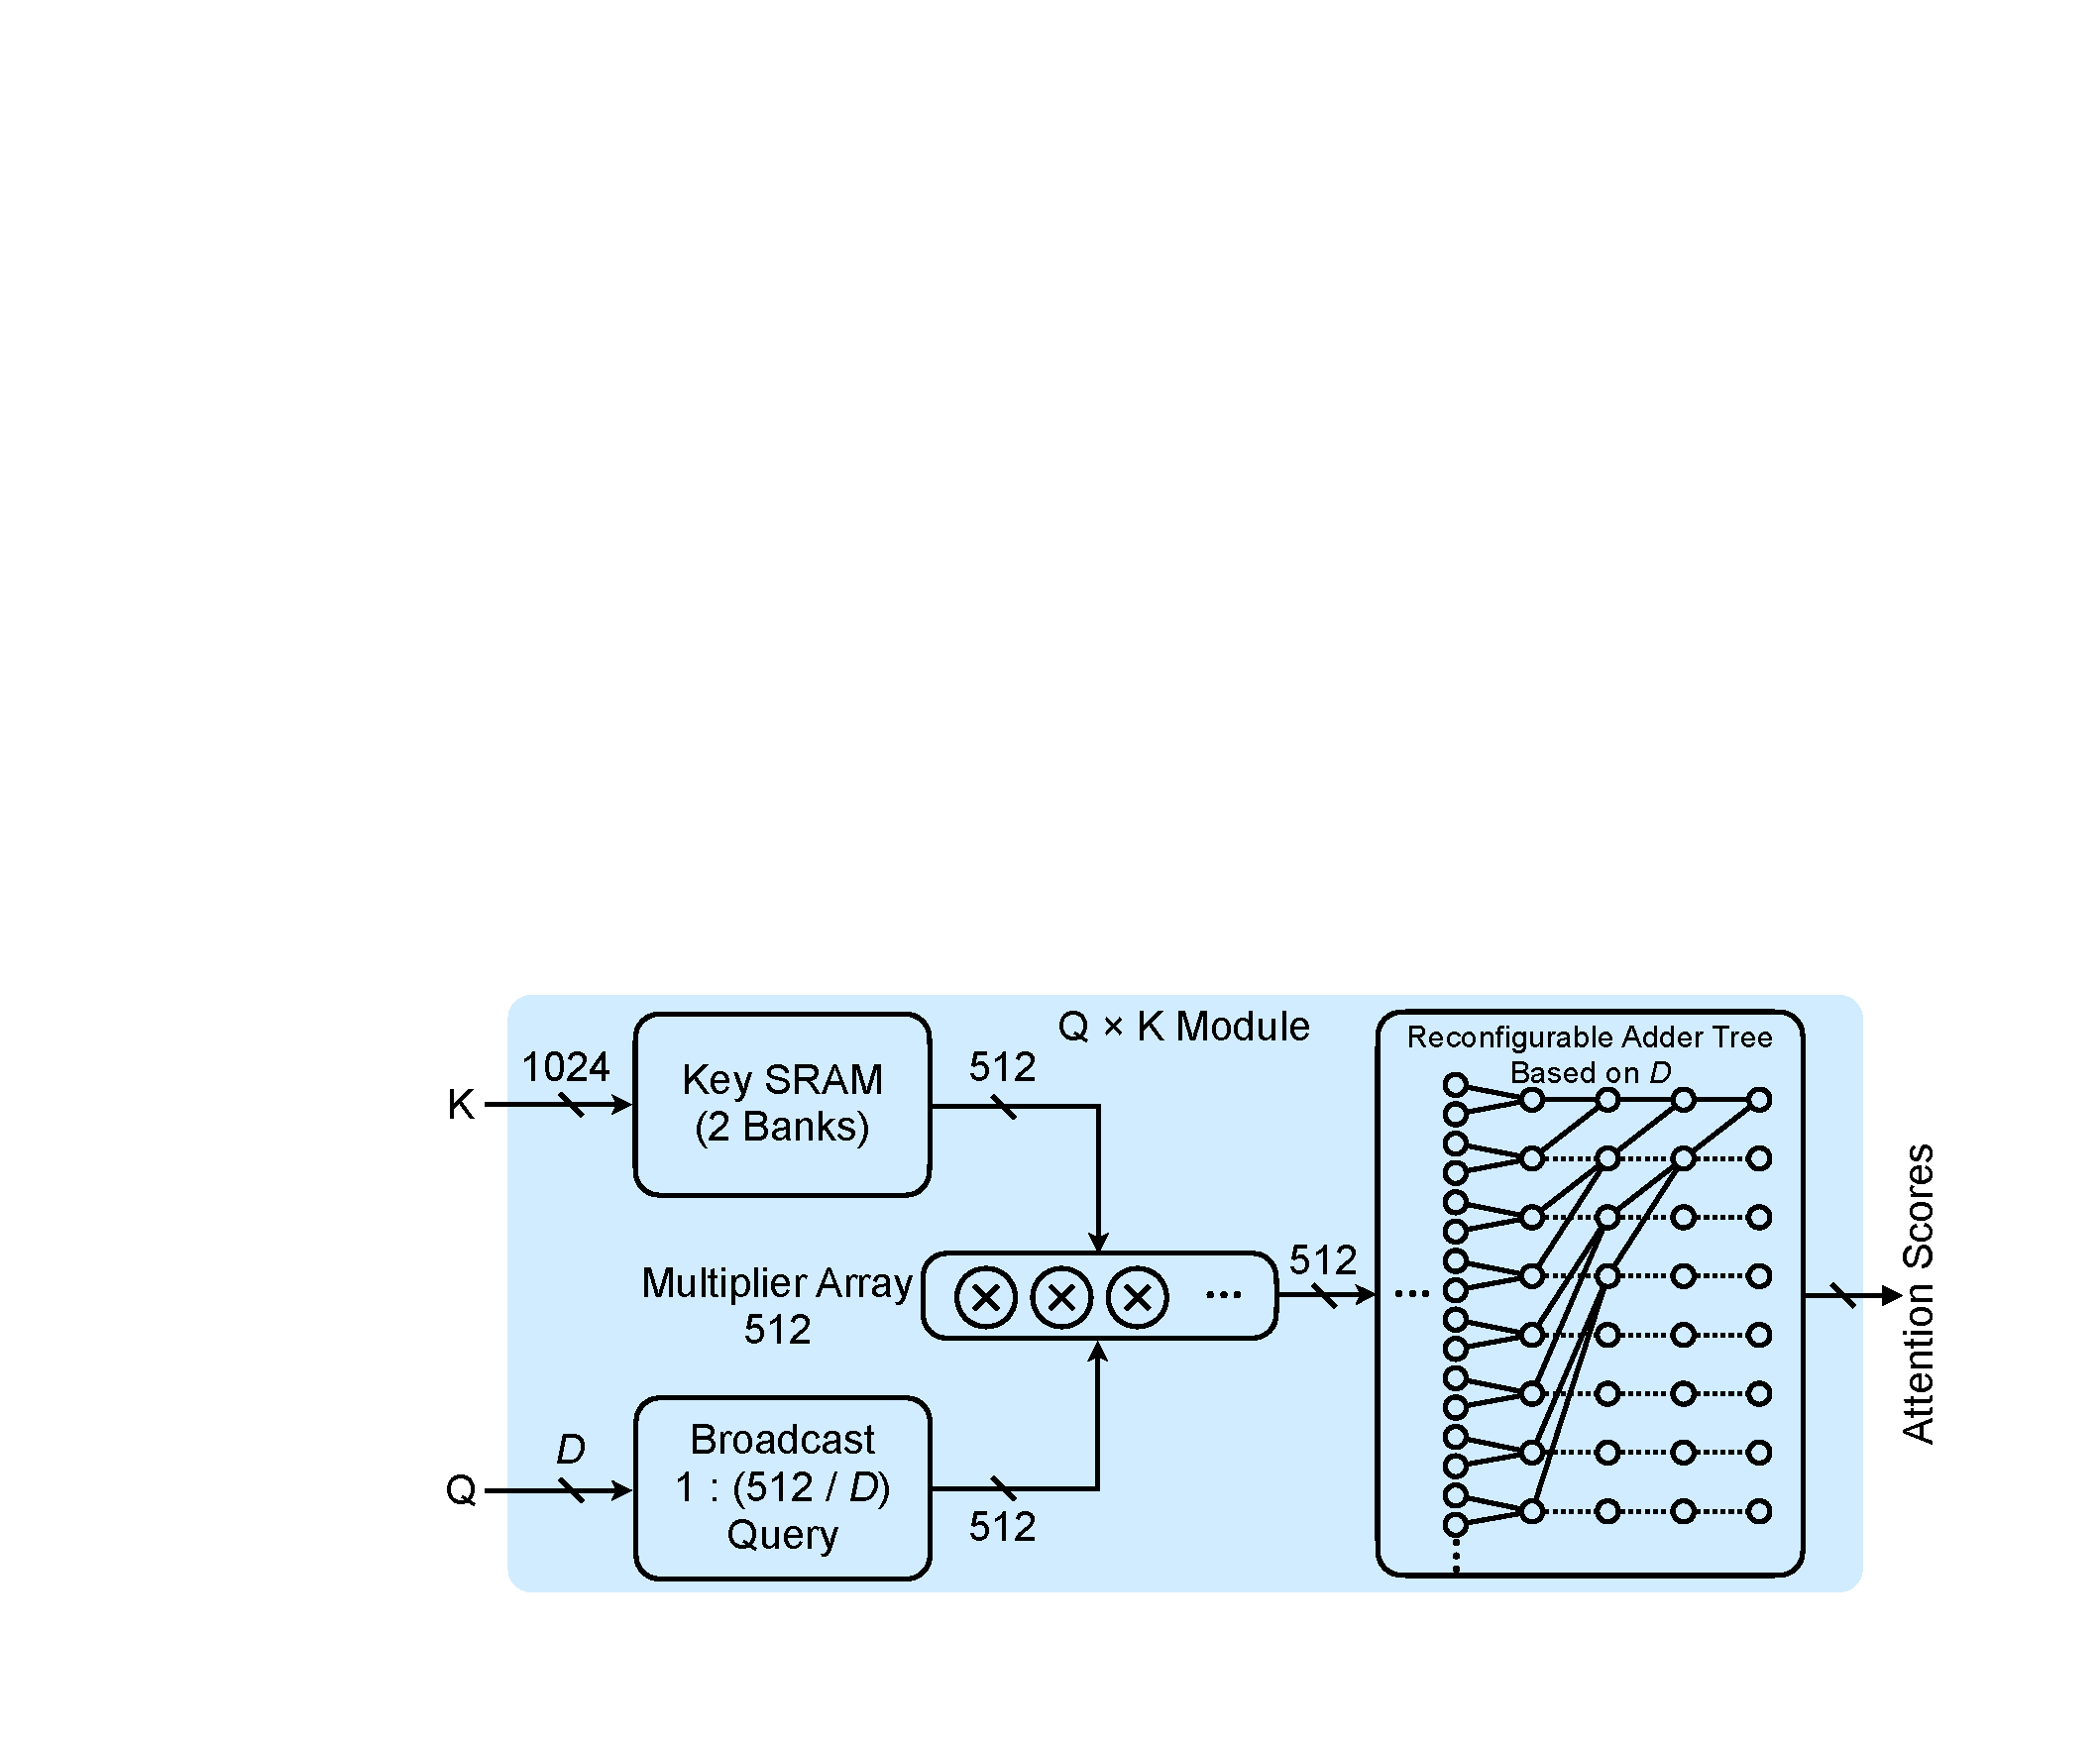
\includegraphics[width=\columnwidth]{figures/qxk.pdf}
    \vspace{-15pt}
    \caption{Query-Key multiplication module with a reconfigurable adder tree. The adder tree can output a various number of partial sums according to the query vector's dimension.}
    \vspace{-15pt}
    \label{fig:qxk}
\end{figure}


\subsection{Data Fetcher and Bitwidth Converter}
The Q-K-V data fetcher is designed to send multiple random read requests per cycle to all 16 HBM channels, where the QKV are interleaved in different channels. We use a 32-to-16 crossbar to route these read requests to the correct channels. The master side is larger than the slave side. There is no memory access conflict because the crossbar generates at most one memory request for each channel at a time.

In order to support progressive quantization but avoid complex logic overheads, we enforce on-chip SRAMs and multipliers to have a fixed bitwidth. We use a bitwidth converter to convert the data loaded from DRAM (4,8,12 bits) uniformly into on-chip bitwidth (12 bits). The converter consists of MUXes to select correct bits from the input and a shifter to allow reading data from an unaligned address.


\subsection{Query-Key Multiplication Module}
The query-key multiplication module (Figure~\ref{fig:qxk}) is designed to calculate the matrix-vector multiplication between K and Q. In each cycle, a row of the key matrix K$_i$ is loaded from the K SRAM, multiplied by Q with a multiplier array, and fed to an adder tree. Adder tree then computes attention scores by reducing all multiplied results $s_i = \sum_j \mathrm{K}_{ij} \times \mathrm{Q}_j$.
We use 512 multipliers in this module to fully utilize the DRAM bandwidth. To support queries and keys with dimension $D$ lower than 512, we get 512/$D$ attention scores in each cycle. The corresponding multiple K$_i$s are packed into the same line in the Key SRAM, and the query is broadcast for 512/$D$ times so that all K$_i$s can have access to the same Q. The adder tree is also configurable to output the results of the last several layers, making it function like 512/$D$ separate D-way adder trees capable of producing multiple results $s_i$.


\subsection{Softmax and Progressive Quantization}
The fixed-point attention scores $s$ from query-key multiplication are first dequantized using a scaling factor. The attention score normalization factor sqrt($D$) is also included in the scaling factor, so that we can perform attention score dequantization and normalization simultaneously. After that, a pipeline of floating-point exponential, accumulation, and division operations are applied to calculate the Softmax results $e^{s_i}/\sum_j e^{s_j}$. The results are finally quantized again so that the operations after Softmax can be performed in fixed-point.

The Softmax results are then fed to the progressive quantization determination module to examine whether LSBs are required. Specifically, we compare the max attention probability with a pre-defined threshold. If smaller than the threshold, the Q-K-V data fetcher will be informed to fetch the LSBs.

\subsection{Attention Prob-Value Multiplication}
The attention prob-value multiplication unit takes the attention probabilities as inputs, multiplies them with the Vs and then accumulates to get attention outputs $A_j = \sum_i attention\_prob_i \times \mathrm{V}_{ij}$. It contains another broadcast-multiply-reduce pipeline, similar to the one in the query-key multiplication module, to support the processing of multiple attention probabilities at the same time. The module has 512 multipliers. The attention probabilities are broadcast for $D$ times, and the adder tree is configured to function like $D$ 512/$D$-way adder trees. The $attention\_out$ are in 12 bits.

\begin{figure}[t]
    \centering
    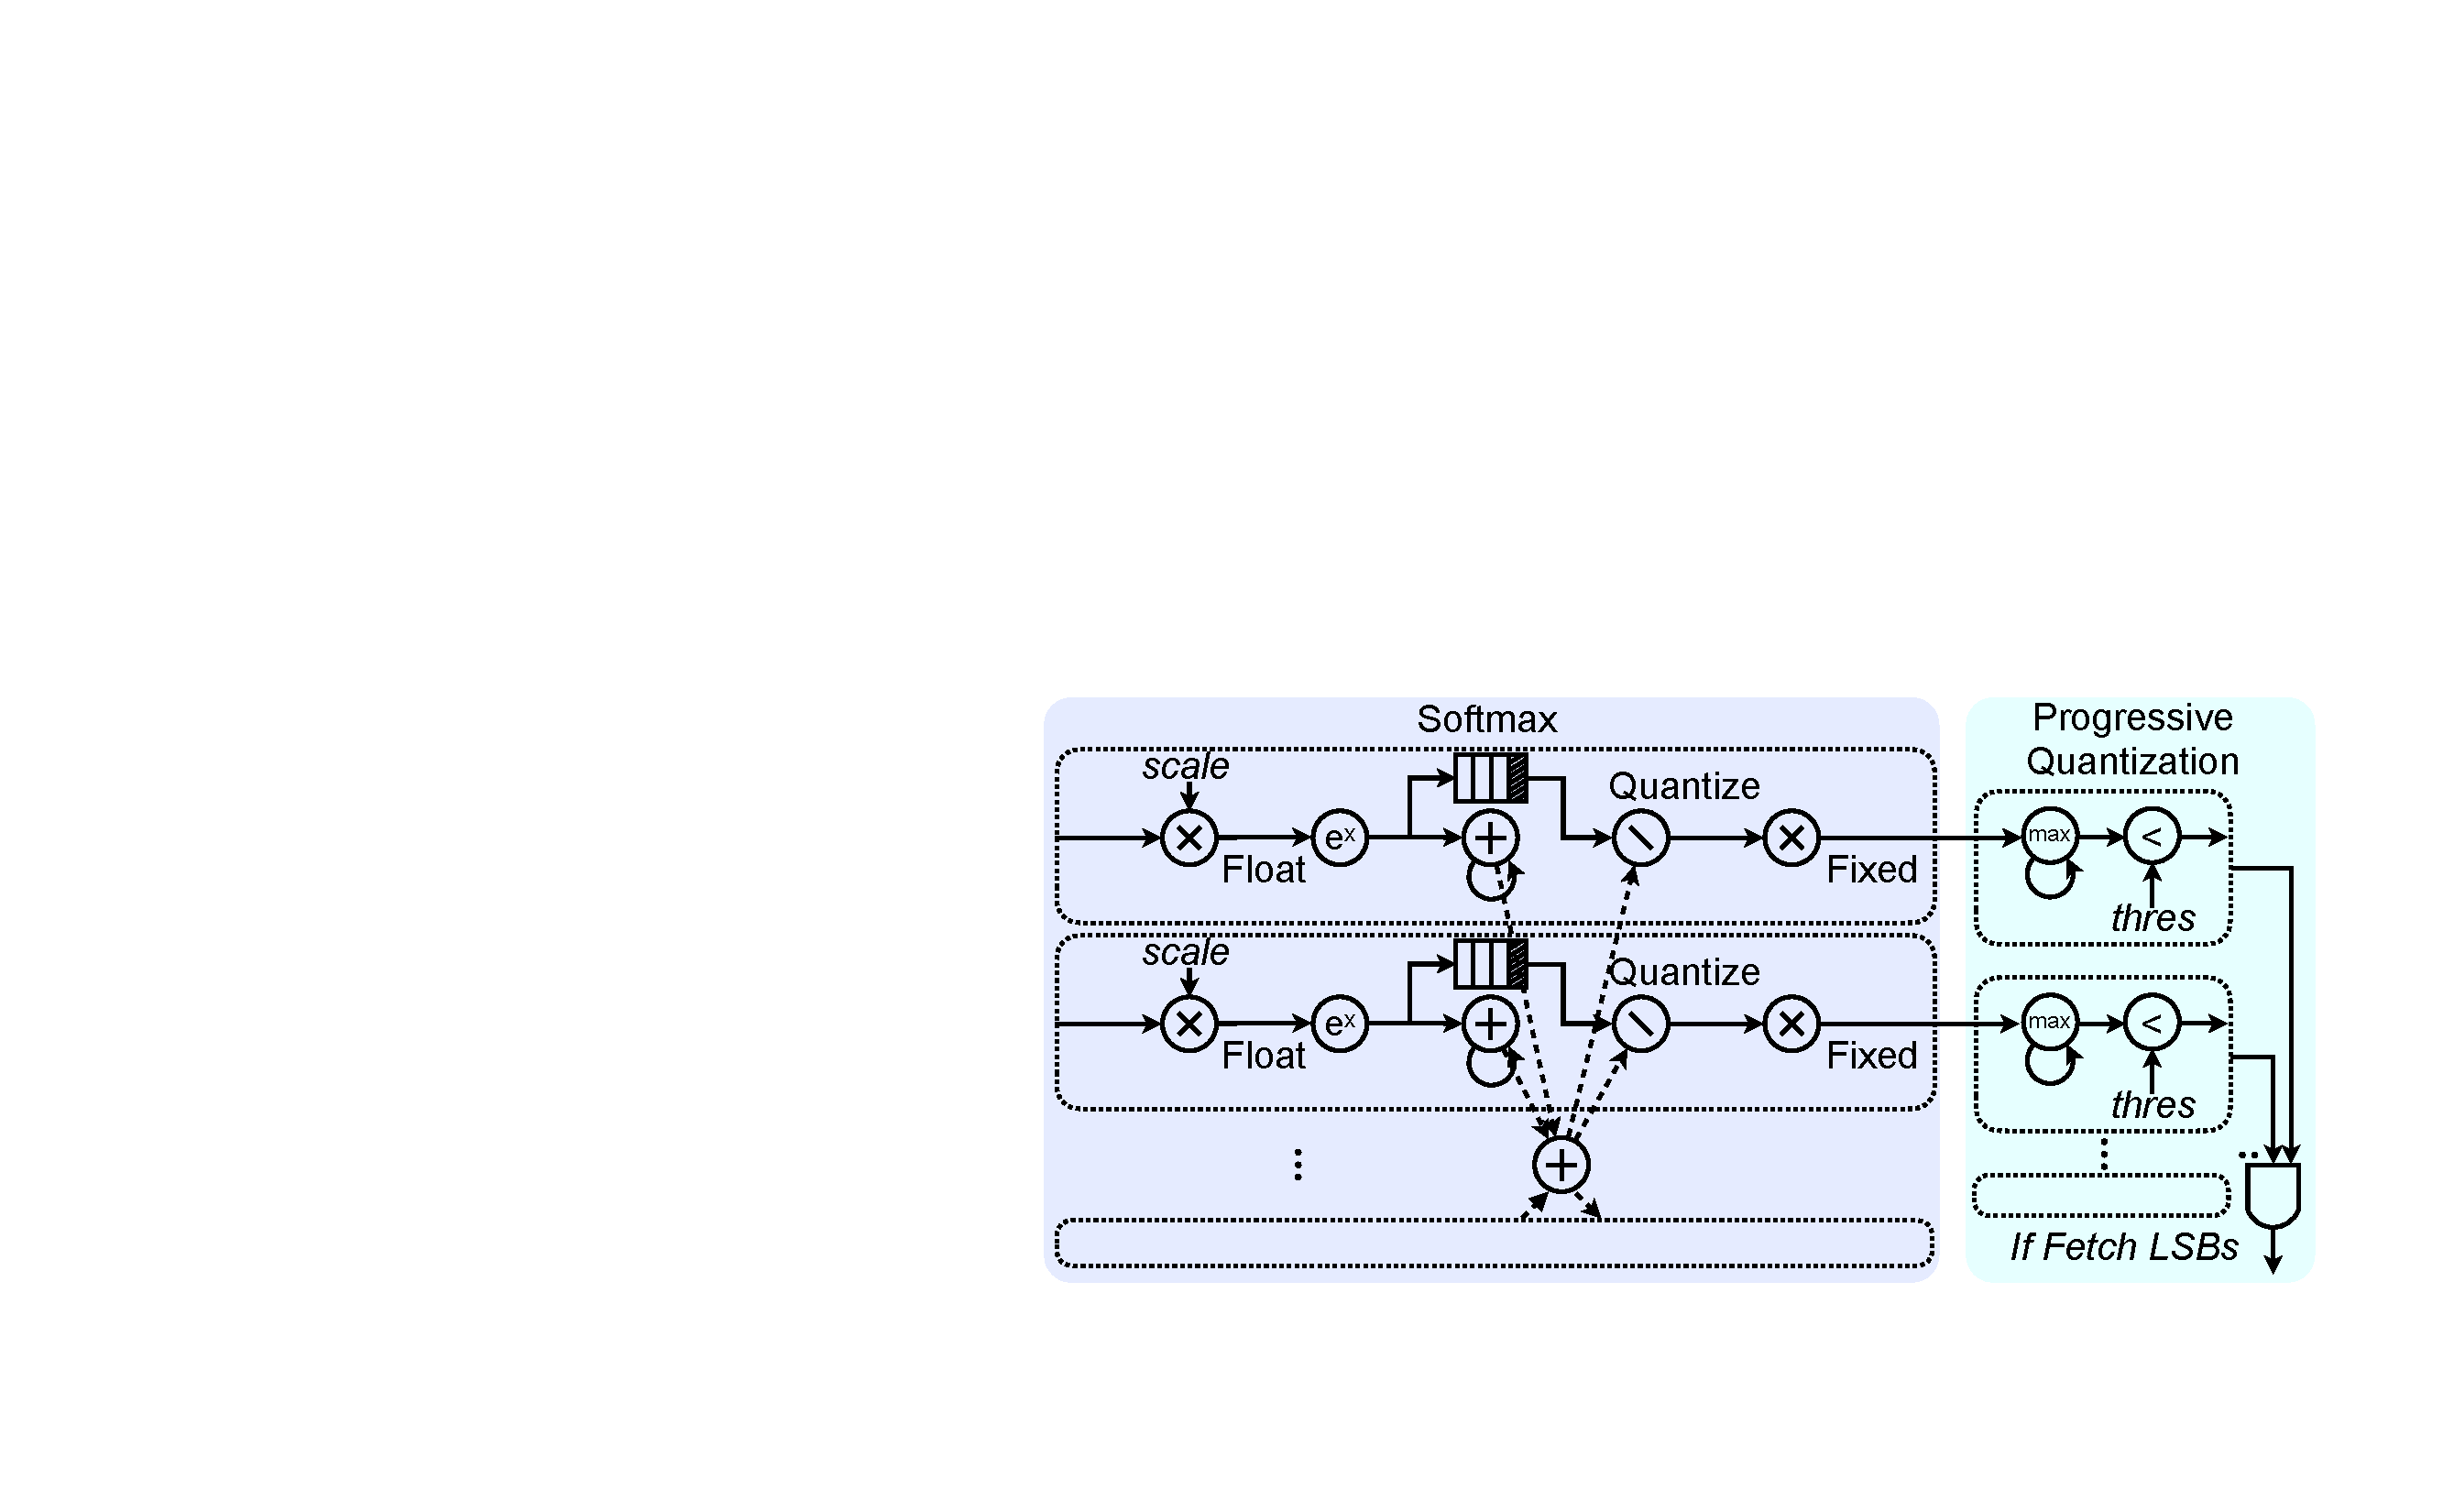
\includegraphics[width=1\columnwidth]{figures/softmax.pdf}
    \vspace{-20pt}
    \caption{Softmax and progressive quantization determination modules.}
    \vspace{-10pt}
    \label{fig:softmax}
\end{figure}

\begin{table}[t]
\renewcommand*{\arraystretch}{0.5}
\setlength{\tabcolsep}{8pt}
\footnotesize
\centering
\caption{Architectural Setups of \spattenfull.}
\vspace{-5pt}
\begin{tabular}{l|l}
\toprule
  \multirow{2}{*}{Q-K-V Fetcher} & A 32$\times$16 address crossbar and a 16$\times$32 \\
   & data crossbar; each port has a 64-depth FIFO. \\ \midrule
 \multirow{2}{*}{Q $\times$ K} & 196KB Key SRAM; 512$\times$12-bit multipliers; \\
 & Adder tree outputs at most 8 items/cycle. \\ \midrule
 Softmax & FIFO depth for softmax: 128; Parallelism: 8. \\ \midrule
 Attention\_Prob $\times$ V & 196KB Value SRAM; 512$\times$12-bit multipliers.  \\ \midrule
 \multirow{3}{*}{HBM} & HBM2, 16$\times$128-bit HBM channels @ 2GHz;\\
 & each channel has 2$\times$64-bit pseudo-channels \\
 & and provides 32GB/s bandwidth. \\
 \bottomrule
\end{tabular}
\vspace{-10pt}
\label{tab:setup}
\end{table}



